\begin{figure}[h!]
	\centering
	\begin{minipage}[b]{1\textwidth}
    		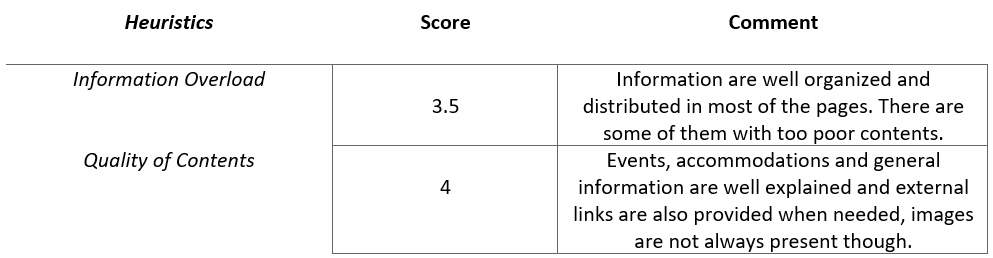
\includegraphics[width=\textwidth]{./assets/contents-final.PNG}
	\end{minipage}
\end{figure}
\FloatBarrier

\subsubsection{Information Overload}
Most of the pages have a balanced quantity of information but some other do not contain any explanation of their contents except for the title. Sometimes the title is enough expressive, but the user experience loses clearness because of the lack of text .
\FloatBarrier

\subsubsection{Quality of Contents}
The overall quality of contents is good: the information is well written and organized  and some nice interactive elements are provided to the user by the leftbar (fig.3); unfortunately some graphical contents are missing, such as some images as in the accomodation element in figure 6.b.
\begin{figure}[h!]
	\subfloat[Accomodation card with complete information]{
		\begin{minipage}[b]{0.48\textwidth}
			\centering
			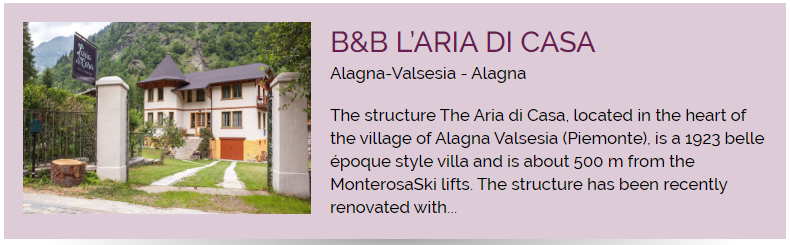
\includegraphics[width=\textwidth]{./assets/bnb-with-image.png}
		\end{minipage}}
		\hfill
	\subfloat[Accomodation card without complete information]{
		\begin{minipage}[b]{0.48\textwidth}
			\centering
			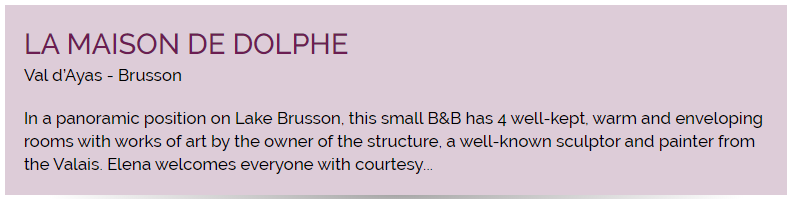
\includegraphics[width=\textwidth]{./assets/bnb-without-image.png}
		\end{minipage}}
		\hfill
	\caption{}
\end{figure}



